\documentclass[a4paper,11pt,leqno]{report}\usepackage[]{graphicx}\usepackage[]{color}
%% maxwidth is the original width if it is less than linewidth
%% otherwise use linewidth (to make sure the graphics do not exceed the margin)
\makeatletter
\def\maxwidth{ %
  \ifdim\Gin@nat@width>\linewidth
    \linewidth
  \else
    \Gin@nat@width
  \fi
}
\makeatother

\definecolor{fgcolor}{rgb}{0.345, 0.345, 0.345}
\newcommand{\hlnum}[1]{\textcolor[rgb]{0.686,0.059,0.569}{#1}}%
\newcommand{\hlstr}[1]{\textcolor[rgb]{0.192,0.494,0.8}{#1}}%
\newcommand{\hlcom}[1]{\textcolor[rgb]{0.678,0.584,0.686}{\textit{#1}}}%
\newcommand{\hlopt}[1]{\textcolor[rgb]{0,0,0}{#1}}%
\newcommand{\hlstd}[1]{\textcolor[rgb]{0.345,0.345,0.345}{#1}}%
\newcommand{\hlkwa}[1]{\textcolor[rgb]{0.161,0.373,0.58}{\textbf{#1}}}%
\newcommand{\hlkwb}[1]{\textcolor[rgb]{0.69,0.353,0.396}{#1}}%
\newcommand{\hlkwc}[1]{\textcolor[rgb]{0.333,0.667,0.333}{#1}}%
\newcommand{\hlkwd}[1]{\textcolor[rgb]{0.737,0.353,0.396}{\textbf{#1}}}%

\usepackage{framed}
\makeatletter
\newenvironment{kframe}{%
 \def\at@end@of@kframe{}%
 \ifinner\ifhmode%
  \def\at@end@of@kframe{\end{minipage}}%
  \begin{minipage}{\columnwidth}%
 \fi\fi%
 \def\FrameCommand##1{\hskip\@totalleftmargin \hskip-\fboxsep
 \colorbox{shadecolor}{##1}\hskip-\fboxsep
     % There is no \\@totalrightmargin, so:
     \hskip-\linewidth \hskip-\@totalleftmargin \hskip\columnwidth}%
 \MakeFramed {\advance\hsize-\width
   \@totalleftmargin\z@ \linewidth\hsize
   \@setminipage}}%
 {\par\unskip\endMakeFramed%
 \at@end@of@kframe}
\makeatother

\definecolor{shadecolor}{rgb}{.97, .97, .97}
\definecolor{messagecolor}{rgb}{0, 0, 0}
\definecolor{warningcolor}{rgb}{1, 0, 1}
\definecolor{errorcolor}{rgb}{1, 0, 0}
\newenvironment{knitrout}{}{} % an empty environment to be redefined in TeX

\usepackage{alltt}

\usepackage{amsmath, amssymb, mdframed, caption, subcaption, graphicx, enumitem, tikz, bbm}
\usepackage{nicefrac}
\usetikzlibrary{bayesnet}

\usepackage{hyperref}
\hypersetup{colorlinks=true, urlcolor=blue, breaklinks=true}

\newmdtheoremenv{Definition}{Definition}[chapter]
\newmdtheoremenv{Exercise}[Definition]{Exercise}
\newmdtheoremenv{Theorem}[Definition]{Theorem}
\newmdtheoremenv{Lemma}[Definition]{Lemma}

\newcommand{\supp}{\operatorname{supp}} 
\newcommand{\E}{\mathbb{E}}
\newcommand{\eps}{\varepsilon}

\newcommand{\id}[1]{\mathbbm{1}\left(#1\right)}

\newcommand{\philip}[1]{ \textcolor{red}{\textbf{Philip:} #1}}
\newcommand{\chris}[1]{ \textcolor{blue}{\textbf{Chris:} #1}}

\title{Basic Probability}
\date{}



\IfFileExists{upquote.sty}{\usepackage{upquote}}{}
\begin{document}

\setcounter{chapter}{5}



\chapter{The EM Algorithm}

\section{Mixture Models}\label{sec:mixtureModels}

In the previous chapter we have mentioned that it may happen that a likelihood function has multiple 
maxima and that sometimes it may be hard or impossible to find the global maximum (i.e.\ the maximum
with the overall highest likelihood value). Such a situation occurs whenever the probabilistic model
that we use to model our observations is a \textbf{latent-} or \textbf{hidden-variable model}. Latent-variable
models are models that besides modelling observed data also model a portion of unobserved data. For
example, if we look at the income distribution of a population we may want to further differentiate
between age groups. If the age of all or some members of the population is not provided in the data, we
can still model it as a latent variable. The difficulty is that we will have to make inferences about the
age of an individual based on other information that we have about it (e.g.\ the income). 

While it may in general be quite hard to formulate latent-variable models, there are certain standard
latent-variable models that have wide-spread applications. One such class are \textbf{mixture models}.

\begin{Definition}[Mixture Model]\label{def:mixtureModel}
We assume jointly distributed random variables $ X=X_{1}^{n} $ and $
Y=Y_{1}^{n} $ where $ Y $ is \href{https://en.wikipedia.org/wiki/Categorical_variable}{categorical} (as defined on Page~\pageref{lab:categorical}) and
$ supp(Y) = \{c_{1}, \ldots, c_{k}\} $. The $ X_{i} $ are observed data, the $ Y_{i} $ are latent
or observed and the $ c_{j}, 1\leq j \leq k $ are called mixture components. 
If the distribution
$ P(X_{1}^{n}=x_{1}^{n}, Y_{1}^{n} = y_{1}^{n}\mid \Theta = \theta) $ factors as
\begin{align*}
&P(X_{1}^{n}=x_{1}^{n}, Y_{1}^{n} = Y_{1}^{n}\mid \Theta = \theta)  \\
&= P(Y_{1}^{n} = y_{1}^{n}\mid \Theta = \theta) \prod_{i=1}^{n} 
P(X_{i}=x_{i} \mid Y_{i} = y_{i}\mid \Theta = \theta) \ .
\end{align*}
we call this model a \emph{mixture model}. The marginal probabilities $ P(Y_{i}=y_{i}) $ for $ 1 \leq i \leq n $ are called
\emph{mixture weights}.
\end{Definition}

Mixture models are extremely useful whenever we have different ways to think about our data. Each way
of conceptualising our data can be encoded by one of the mixture components of the mixture model. The modelling
of the data under that view is done by the conditional distribution induced by the mixture component.
This technique can help us to build a better overall model of our data. Let us introduce a running example that
we use for the rest of this section. A graphical depiction of the model used in the example is given in Figure~\ref{fig:mixtureGraphical}.

\paragraph{Notation} Notice that throughout this chapter we use $ \Theta $ as a generic variable over collections of parameters. Assume any
model that has parameters $ p $ and $ q $. Then we have $ \Theta = (p,q) $. For the time being you can thus regard the conditioning on $ \Theta = \theta $
as an underspecified dependence on any parameters that the model may have. We will become more concrete about parameter values in Section~\ref{sec:EMExample}.
\begin{figure}
\center
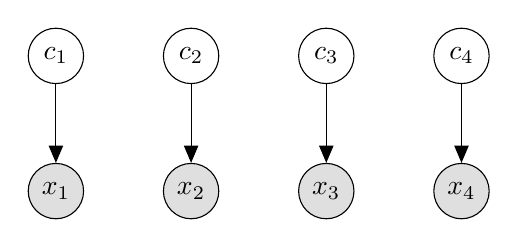
\begin{tikzpicture}
\node[latent] 					(c1)		{$ c_{1} $};
\node[latent, right = of c1] 	(c2) 	{$ c_{2} $};
\node[latent, right = of c2] 	(c3) 	{$ c_{3} $};
\node[latent, right = of c3] 	(c4) 	{$ c_{4} $};

\node[obs, below = of c1] (x1) {$ x_{1} $};
\node[obs, below = of c2] (x2) {$ x_{2} $};
\node[obs, below = of c3] (x3) {$ x_{3} $};
\node[obs, below = of c4] (x4) {$ x_{4} $};

\edge{c1}{x1};
\edge{c2}{x2};
\edge{c3}{x3};
\edge{c4}{x4};
\end{tikzpicture}
\caption{A graphical model of the mixture model used in our
  example. Only four data points are shown. Shaded nodes indicate observed values, light nodes indicate
latent values. A graphical model shows the dependencies between variables in a probabilistic model. In this example we see that a) the latent variables
are independent of each other and b) the observed variables are independent given the latent variables. (Aside: formally the graphical model actually shows the
\textit{independencies} assumed by our model! Reasoning about it in terms of dependencies is often easier, though.)}
\label{fig:mixtureGraphical}
\end{figure}

\paragraph{Example of a mixture model} Assume we observe 20 sequences of coin tosses. Each sequence
contains 10 flips. We also know that there are 3 coins with which these sequences could possibly have been
generated and for each sequence a different coin may have been used. We want to find out what the biases
of the coins are (i.e.\ the parameters of the binomial distributions associated with the coins) and the probability
for each coin to have generated a particular sequence.
 
We could assume that the entire data set was generated by exactly one coin. We would then employ maximum likelihood estimation 
to find the parameter of that coin. However, this model might actually turn out to be
pretty bad because we are committing to picking one coin only. This is
a bad assumption, because we know that each sequence may have been generated by a different coin. 

A mixture model comes to the rescue. Instead of assuming that only one coin has generated all 20 sequences,
we assume that all three coins have contributed to generating the 20 sequences. However, their contributions
may not be equal. This inequality is exactly what the mixture weights capture. 

In order to model the contribution of each coin, we introduce a latent RV $ Y $ over mixture components with labels $ c_{1}, c_{2}, c_{3} $ representing the three coins.
In the present case, each mixture component is linked to a binomial distribution, parametrized by the biases of
the coins. We will also adopt the often-used assumption
that the mixture components are independent of each other. This means that the coin that generated each
sequence of coin flips was chosen independently of the coins used for the other sequences. Our independence assumptions
are also encoded in the graphical model in Figure~\eqref{fig:mixtureGraphical}. As usual, we call our data $ x $. 
This information suffices to formulate our mixture model.
\begin{align} 
&P(X_1^n=x_{1}^{n},Y_{1}^{n}=y_{1}^{n}\mid \Theta=\theta) \label{eq:mixtureExample} \\
&= \prod_{i=1}^{n} P(Y_{i}= y_{i} \mid \Theta=\theta)P(X_{i}=x_{i} \mid Y_{i}=y_{i},\Theta=\theta) \nonumber 
\end{align}

Notice that if we were given the mixture weights, estimating
the parameters of the mixture components would be easy: we would simply find the MLE for each mixture component separately. The mixture
model could then easily be constructed because the mixture weights are known. 

Usually, we face a more difficult problem when working with mixture models. Neither the mixture
weights nor the parameters of the mixture components are known. In this case, doing straighforward MLE is impossible because the data is
incomplete\footnote{Incomplete data is 
  another name for a collection of random variables of which some have unobservable (latent) outcomes. Data modelled with a mixture model is incomplete because it contains
  an observed part (the number of heads in our example) and a latent
  part (the mixture components which in our example are the types of coin). In general, whenever you have complete data, analytic MLE computation is possible. The moment your data is incomplete, it becomes impossible.}. 

How can we go about estimating the model parameters, i.e.\ the parameters of the mixture components and the mixture weights?
Each factor
in \eqref{eq:mixtureExample} is in fact a joint distribution (by the chain rule). We exploit this to rewrite the model as a model of the
observed data only.
%\begin{align}\label{eq:marginal}
%P(X_1^n=x_{1}^{n} \mid  \Theta= \theta) &= \prod_{i=1}^{n} \sum_{j=1}^{3} P(X_{i}=x_{i},Y_{i}=c_{j} \mid  \Theta= \theta)
%\end{align}
%\philip{Compare this to Equation~\eqref{eq:mixtureExample}. There we constructed a probability distribution over the joint outcomes $ X_{1}^{n} $ and
%$ Y_{1}^{n} $. Because we assumed independence between mixture components, the distribution could be factorised over pairs $ (X_{i},Y_{i})$ for $ 1 \leq i \leq n $.
%In Equation~\eqref{eq:marginal} we then inferred the marginal distribution for $ X_{1}^{n} $. Recall that in order to compute the marginal of $ X_{1}^{n} $ we
%need to sum over all possible $ Y_{1}^{n} $. Because their joint distribution factorises nicely, we can perform the marginalisation per $ (X_{i},Y_{i})$ pair.
%This is exactly what is happening in Equation~\eqref{eq:marginal}. 
%Please pay attention to a crucial notational difference between \eqref{eq:mixtureExample} and
%\eqref{eq:marginal}: In the former we wrote $ Y_{i}=y_{i} $ whilst in the latter we wrote $ Y_{i}=c_{j} $. Why did we do this? Equation~\eqref{eq:mixtureExample} is
%a joint distribution and thus $ Y_{i} $ needs to take on a \textit{specific} value $ y_{i} \in \{c_{1},c_{2},c_{3}\} $. To get the marginal distribution of
%$ X_{i} $, however, we need to sum over \textit{all} values that $ Y_{i} $ can take on. We do this by writing $ Y_{i} = c_{j} $ which provides us with a means
%of summing over the possible outcomes $ c_{1},c_{2},c_{3} $.}
%\chris{this is going too fast! I don't understand it, you also
%  switched from $y_1^n$ to $c_j$ somehow... where did you use
%  \eqref{eq:mixtureExample} here??}\philip{Sorry, the conditioning was wrong in 6.1. Please check whether the above explanation helps you to understand what's going
%  on now.}
% \begin{align}\label{eq:marginal}
% P(X=x_{1}^{n} \mid  \Theta= \theta) &= \sum_{j=1}^3 P(Y_i = c_j)
%                                  P(X=x_{1}^{n} \mid Y_{1}^{n}=y_{1}^{n},\Theta=\theta)
%   \\
% &=  \prod_{i=1}^{n} \sum_{j=1}^{3} P(X_{i}=x_{1},Y_{i}=c_{j} \mid  \Theta= \theta)
% \end{align}

\begin{align}
P(X_1^n=x_{1}^{n} \mid \Theta= \theta) &= \sum_{j_1=1}^3 \sum_{j_2=1}^3 \cdots \sum_{j_n=1}^3 P(X_1^n=x_{1}^{n}, Y_1=c_{j_1}, \ldots, Y_n=c_{j_n} \mid \Theta= \theta) \label{eq:marginal} \\
&= \sum_{j_1=1}^3 \sum_{j_2=1}^3 \cdots \sum_{j_n=1}^3 \prod_{i=1}^{n} P(X_{i}=x_{i},Y_{i}=c_{j_i} \mid  \Theta= \theta) \nonumber \\
&= \prod_{i=1}^{n} \sum_{j=1}^3 P(X_{i}=x_{i},Y_{i}=c_{j} \mid  \Theta= \theta) \, , \nonumber
\end{align}
where the second equality uses the fact that we have assumed independence between the mixture components and hence
the expression $P(X_1^n=x_1^n, Y_1^n=y_1^n \mid \Theta = \theta)$ factorizes.
Now that we have related mixture models to the probability of the observed data, we can hope to estimate
their parameters using the maximum-likelihood principle.

There is one remaining problem, however: if the mixture weights $P(Y_i=y_i)$ are unknown, there is no closed-form solution for estimating the likelihood function. This is because
the likelihood depends on the parameters of the mixture components whose distribution, given
by the mixture weights, is unknown. This means that while we can compute the likelihood for each
individual mixture component, we cannot compute the likelihood of the entire mixture model because we
do not know how much each component contributes to the overall likelihood term. As a consequence, we can not 
simply apply calculus as we have been doing up to now. For this reason, we turn to the \textbf{EM algorithm}, 
that allows to at least find a local maximum of the likelihood function.

One final note: At the beginning we introduced latent-variable models (and hence mixture models) as models
of \textit{latent data}. We have cast the problem of inferring the mixture weights as inferring a 
distribution over mixture components, however. One may argue that those are not data, neither latent nor 
observed. This is a fair criticism but there is an easy way out. Simply imagine that each sequence of coin
flips was annotated with a pointer to the mixture component (the coin) that generated it. This annotation
is clearly part of the data. Since in our actual data, these annotations are missing, we treat them as 
latent data.

\section{The EM Algorithm}

In order to estimate the parameters of mixture models, we can employ a classical algorithm of 
\textbf{unsupervised learning}\footnote{Whenever the feature of our
  data that we want to predict (such as the coin which generated a sequence)
is observed, we speak of supervised learning. If the target feature is latent, we speak of unsupervised learning.}, 
namely the \textbf{expectation-maximisation (EM) algorithm}. This
algorithm allows to find a local maximum of the likelihood function of mixture models or, more
generally, models with missing data. 

\paragraph{Another example of latent data.} To give you some more intuition for what latent data is we provide a further example that has
spawned a lot of research. Assume you run a website that recommends movies
based on a user's preferences. In order to make statistical predictions about what type of user
likes what kind of movie, you ask your users to rate movies according to different categories.
Say you ask your users to rate the movies for entertainment value, action and fun. What may happen is
that some of your users only rate a movie in one or two of these three categories. However, these
ratings are still valuable to you and you do not want to throw them away, just because the rating is
incomplete. Thus you have a data set with some missing data that you have to fill in somehow.
\bigskip

In mixture models, annotations that tell you which mixture component
generated a given data point can be thought of as missing data. As we have seen, such annotations
are usually missing and thus we cannot do maximum likelihood estimation. The idea of EM is to
make an educated guess at the probability with which each mixture component could \textit{potentially}
have generated a data point $ x_{i} $. What we do know is our observed data and some initial guess of the mixture
weights which act as prior probabilities for the mixture components (this guess may be arbitrary). 
Our educated guess is then simply based on Bayes' rule. It is the posterior probability of each mixture
component given the data point $ x_{i} $.

Using the posterior over the latent (missing) data, the EM algorithm allows us to probabilistically fill in the missing data and find good mixture weights
(where you should understand \textit{good} in the maximum-likelihood sense). The idea behind the
algorithm is simple: first, compute the expected number of occurrences of the missing data values (the mixture 
components). Then treat these expectations as observed and do maximum likelihood estimation as usual\footnote{Notice that expectations can take on non-integer values and thus when treating them as observations we are handling a dataset with ``fractional'' observations. While this may be conceptually awkward
it does not change the mathematics of maximum likelihood estimation.}. Repeat the procedure 
until the likelihood does not increase any further. Notice that this procedure requires to
fix the number of mixture components in advance.

More formally, assume a data set $ X=x $. Furthermore, define $ Y $ as a random variable over latent data that can
take on $ |\mathcal{Y}| $ possible values $c_1, c_2, \ldots, c_{|\mathcal{Y}|}$. Then the likelihood function is 
\begin{align}
L_{x}(\theta) = P(X=x \mid \Theta=\theta) = \underset{j=1}{\overset{|\mathcal{Y}|}{\sum}} P(X=x, Y=c_{j} \mid \Theta=\theta)
\end{align}
where $ \Theta $ ranges over the parameters of the joint distributiforon $ P_{XY} $. Recall that EM
probabilistically fills in missing data. However, since we are doing maximum likelihood estimation, we
are not so much interested in the missing data itself but rather in the sufficient statistics of
that data (see Section~\ref{sec:sufficientStats}). Since we cannot directly obtain the sufficient statistics
of missing data, we will instead compute the \textit{expected sufficient statistics}\footnote{
Because we are referring to sufficient statistics our exposition of EM is specific to distributions
in the exponential family. The EM algorithm can also be made more general. However, since virtually
all distributions of interest in practice do belong to the exponential family, we will not make this kind of generalisation.
}.

The EM algorithm is an iterative 
algorithm, meaning we repeat its steps several
times. We use superscripts to indicate the number $l$ of the repetition, where $ 0 \leq l \leq k $.
To formalize the EM algorithm, assume we are at iteration $l$ for which we have some parameter estimate 
$\theta^{(l)} $ (the initial estimate $\theta^{(0)}$ can be set arbitrarily). Based on this parameter 
estimate we then compute the expected sufficient statistics of our model which we will call $ t(y,x) $.
\begin{equation} \label{Estep}
t(y,x)^{(l+1)} = \E(t(Y,x) \mid X = x,\Theta = \theta^{(l)})
\end{equation} 
%\chris{would it make sense to always write $\E_Y(\ldots)$ to indicate where the expectation is taken over?}\philip{Yeah, I guess we could do that. Do you think we'd have
%to explain that kind of notation or would people understand it?}

Equation~\eqref{Estep} is known as the \textbf{E(xpectation)-step} of the EM algorithm. This name
comes from the fact that in this step we compute the expected sufficient statistics. 
To make the algorithm complete, we still miss a
\textbf{M(aximization)-step}. But that step is simple. We pretend that the expected sufficient statistics of 
the latent data were actually observed. Once we pretend to observe the expected statistics, the maximization 
step can be performed using the maximum-likelihood estimation:
\begin{equation} \label{Mstep}
\theta^{(l+1)} = \underset{\theta}{\arg\max} \, P(X=x, t(Y,X) = t(y,x)^{(l+1)} \mid \theta)
\end{equation}

\begin{Definition}[EM algorithm]\label{def:EM}
We assume a data set $ x $ and postulate that there is unobserved data $ y $. We also
assume a probabilistic model $ P(X=x,Y=y \mid \Theta = \theta) $ whose parameters are realisations of a RV
$ \Theta $. Let $ t(x,y) $ be the sufficient statistics for that model. Then any
iterative algorithm with $ m $ iterations that performs the following
steps for $0\leq l \leq m-1$, 
\begin{align*}
\mbox{\textbf{E-step:} } \quad t(y,x)^{(l+1)} &= \E(t(Y,x) \mid X = x, \Theta = \theta^{(l)}) \\
\mbox{\textbf{M-step:} } \qquad \theta^{(l+1)} &= \underset{\theta}{\arg\max} \; P(X=x, t(Y,X) = t(y,x)^{(l+1)} \mid \Theta = \theta) 
\end{align*}
to update the model parameters is called an EM algorithm. 
\end{Definition}

\section{Example of an EM Algorithm for a Mixture Model}\label{sec:EMExample}

Assume as in Section~\ref{sec:mixtureModels} that our data is $ x=x^{20}_{1} $ where each $ x_{i} $ is the 
number of heads that we observed in a sequence of a 10 coin tosses. Again we also assume mixture components representing three coins which are linked
to binomials with parameters representing the biases of the coins. 
The latent data in this case is an annotation that for each observed sequence $ x_{i} $ reveals the coin that has been used
to generate that sequence. Thus we have latent data $ y=y_{1}^{n} $ where each $ y_{i} $ can be one of the three mixture components. 
We make the additional assumption that choosing a coin to generate a particular sequence is done independently of the coins chosen
to generate all the other sequences. This has the effect that in our model the latent data points will be independent\footnote{The assumption
that the mixture components in a mixture model are independent is actually quite common.}.

In this example, our collection of parameters $ \theta $ consists of two group of parameters, namely $ w_{1}, w_{2}, w_{3} $ for the mixture
weights and $ \phi_{1}, \phi_{2}, \phi_{3} $ which are the parameters of the binomials linked to the mixture components (i.e. these parameters
represent the biases of the coins). When we condition on $ \theta $, we will often not need all of the parameters in the collection. For example,
\begin{align*}
P(Y=c_{1}|\Theta=\theta) = P(Y=c_{1}|W_{1}=w_{1}) = w_{1}
\end{align*}
because the first mixture weight is the only parameter that is needed to compute 
the probability of observing the mixture component $ c_{1} $. 

Notice that because the mixture components are categorically distributed we have the constraint that
$ w_{1} + w_{2} + w_{3} = 1 $. Furthermore because $ \phi_{1}, \phi_{2}, \phi_{3} $ are binomial parameters, we know that they have to lie in $ [0,1] $.

\paragraph{E-step} Initially we arbitrarily assume that the coins have biases of $ 0.4, 0.5  $ and $ 0.65 $, meaning that we initialize the binomial parameters of the data-generating
distributions as follows:
\begin{equation}
\phi^{(0)}_{1} = 0.4 \hskip 0.5cm  \phi^{(0)}_{2} = 0.5 \hskip 0.5cm  \phi^{(0)}_{3} = 0.65
\end{equation}
We also assume that the fair coin is more likely to be used and hence set its initial mixture weight to $ w_2^{(0)}=0.5 $ and the mixture weights of the 
other two coins to $ w_1^{(0)}=w_3^{(0)}=0.25 $ (any other choice would also be fine). Let 
us take a closer look at our data. To shorten notation, we write it as a list where the i$ ^{th} $ entry is the value of $ x_{i} $.
$$ \left[ 6, 5, 4, 2, 2, 6, 5, 5, 4, 2, 5, 2, 4, 4, 6, 4, 5, 6, 3, 3 \right] $$ 
Then for each $ x_{i} $ we check how likely each coin is to have generated that point. In order to compute the posterior for each coin given a data point, we need
the likelihood for that data point. For the first observation we get the following likelihood values.


\begin{align}
&P(X_{1}=6 \mid Y_{1} = c_{1}, \Theta=\theta^{(0)}) = P(X_{1}=6 \mid Y_{1}=c_{1},\Phi_{1} = 0.4) = 0.1114767& \\
&P(X_{1}=6 \mid Y_{1} = c_{2}, \Theta=\theta^{(0)}) = P(X_{1}=6 \mid Y_{1}=c_{2},\Phi_{2} = 0.5) = 0.2050781& \nonumber \\ 
&P(X_{1}=6 \mid Y_{1} = c_{3}, \Theta=\theta^{(0)}) = P(X_{1}=6 \mid Y_{1}=c_{3},\Phi_{3} = 0.65) = 0.2376685& \nonumber
\end{align}

Recall that the mixture weights are nothing else than priors over mixture components. Hence, in order to get the joint distribution over observed and
latent data, we multiply the likelihoods by the mixture weights.
\begin{align}
&P(X_{1}=6,Y_{1} = c_{1}\mid \Theta=\theta^{(0)}) = 0.25 \times P(X_{1}=6 \mid Y_{1}=c_{1},\Phi_{1} = 0.4) = 0.0278692 \\
&P(X_{1}=6,Y_{1} = c_{2}\mid \Theta=\theta^{(0)}) = 0.5 \times P(X_{1}=6 \mid Y_{2}=c_{2},\Phi_{2} = 0.5) = 0.1025391 \nonumber \\ 
&P(X_{1}=6,Y_{1} = c_{3}\mid \Theta=\theta^{(0)}) = 0.25 \times P(X_{1}=6 \mid Y_{3}=c_{3},\Phi_{3} = 0.65) = 0.0594171 \nonumber
\end{align}

We are ultimately interested in the posterior over mixture components. Because we are dealing with a categorical
distribution here, the posterior probability is exactly the expected
number of times that each coin has generated data point $ x_{1} $. This is to say that
$\E[\id{Y=c_{j}}\mid X_{1}=6, \Theta = \theta^{(0)}] = P(Y_{1}=c_{j} \mid X_{1}=6, \Theta=\theta^{(0)}) $\footnote{We use
the function $ \id{\cdot} $ as an indicator function that evaluates to 1 whenever its boolean argument is true and to 0 otherwise.}. The
posterior given $ X_{1}=6 $ is shown in Equation~\eqref{eq:posterior}. Recall that we can compute the denominator in Bayes rule (a.k.a.
the marginal likelihood) using marginalisation. For example
\begin{align*}
P(X_1 = 6 \mid \Theta= \theta^{(0)}) = \sum_{i=1}^{3} P(X_{1}=6,Y_{1} = c_{i} \mid \Theta= \theta^{(0)}) \ .
\end{align*} 
%Compute index of first data point in list of ordered outcomes

\begin{align}\label{eq:posterior}
P(Y_{1} = c_{1} \mid X_{1}=6,\Theta= \theta^{(0)}) &= \frac{P(X_{1}=6,Y_{1} = c_{1} \mid \Theta= \theta^{(0)})}{P(X_1 = 6 \mid \Theta= \theta^{(0)})} = 0.1468149 \\
P(Y_{1} = c_{2} \mid X_{1}=6,\Theta= \theta^{(0)}) &= \frac{P(X_{1}=6,Y_{1} = c_{2} \mid \Theta= \theta^{(0)})}{P(X_1 = 6 \mid \Theta= \theta^{(0)})} = 0.5401758 \nonumber \\
P(Y_{1} = c_{3} \mid X_{1}=6,\Theta= \theta^{(0)}) &= \frac{P(X_{1}=6,Y_{1} = c_{3} \mid \Theta= \theta^{(0)})}{P(X_1 = 6 \mid \Theta= \theta^{(0)})} = 0.3130094 \nonumber
\end{align}

We compute these expectations over mixture components for each data point and add them up. The reason we can simply add the expectation is that
the latent variables are independent and consequently their expectations are independent. If this was not the case, simple adding would not
be possible. How exactly the expectations can be accumulated depends on how the model's distribution over latent variables factorises. This has to
be handled on a case-by-case basis. For our examples the expectations for each outcome can be found in Table~\ref{tab:posteriors}.

Once the expectations have been added, we need to compute the sufficient statistics for our model. First of all notice that we are dealing with
a mixture model where the latent variables are always categorical. Thus, in order to update the parameters of $ P_{Y} $ we need to find the
sufficient statistics for a categorical distribution. Recall that these sufficient statistics are simply the counts per outcome observed in
the data. Thus the expected sufficient statistics for a categorical are the expected counts per outcome. But these are simply the posterior
probabilities! Thus we need to multiply the posteriors per of each observed outcome with the number of times this outcome was
seen in the data and sum over all observed outcomes. For mixture component $ c_{1} $ (the first coin with parameter $ \phi^{(0)}_{1} = 0.4 $) this gives
\begin{align}
\E(\id{Y = c_{1}} \mid X=x,\Theta= \theta^{(0)}) = 4 \times 0.5674795 + 2 \times 0.4568744 \label{eq:c1Expectation} \\ 
+ 5 \times 0.3436451 + 5 \times 0.237068 + 4 \times 0.1468149 = 6.6744913 \nonumber \ .
\end{align}
By parallel calculations we get $ \E(\id{Y = c_{2}}\mid X=x,\Theta= \theta^{(0)}) = 10.5237552 $ and $ \E(\id{Y = c_{3}}\mid X=x,\Theta= 
\theta^{(0)}) = 2.8017535 $. 
These are our expected sufficient statistics. Importantly, we get 
$ \E[\id{Y = c_{1}}\mid X=x,\Theta= \theta^{(0)}] + \E[\id{Y = c_{2}}\mid X=x,\Theta= \theta^{(0)}] + \E[\id{Y = c_{3}}\mid X=x,\Theta= \theta^{(0)}] \approx 20 $ (there is some slight numerical imprecision
caused by our computer). Notice that this is a useful debugging technique when implementing the algorithm: if the expected number of mixture components
does not add up to the number of latent variables in your model, then you almost certainly have a bug in your code!
\begin{table}
\center

\begin{tabular}{c|c|c|c|c}
\hline
outcome & occurrences & c\_1 & c\_2 & c\_3\\
\hline
2 & 4 & 0.5674795 & 0.4124300 & 0.0200905\\
\hline
3 & 2 & 0.4568744 & 0.4980674 & 0.0450583\\
\hline
4 & 5 & 0.3436451 & 0.5619435 & 0.0944114\\
\hline
5 & 5 & 0.2370680 & 0.5814960 & 0.1814361\\
\hline
6 & 4 & 0.1468149 & 0.5401758 & 0.3130094\\
\hline
\end{tabular}


\caption{Posteriors per outcome for the mixture components of the coin flip data set from our EM example.}
\label{tab:posteriors}
\end{table}

Next we turn to the sufficient statistics for the binomial distributions linked to the mixture components. These are the counts of the observed outcomes. However,
since the binomials are conditional distributions (they are conditioned on the identity of the coins), the counts have to be taken with respect to their conditioning
contexts. In other words: we cannot count the observed outcomes independently but we have to count pairs of observed and latent variables. Formally this means that 
for one binomially distributed observation $ x_{i} $ the expected number of times that we see the
pair $ (x_{i},c_{j}) $ is $ \E[\id{x_{i},c_{j}} \mid \Theta=\theta^{(0)}] = P(Y_{i}=c_{j} \mid X_{i}=x_{i}, \Theta=\theta^{(0)}) $. This is again
just the posterior that we find in Table~\ref{tab:posteriors}. 

To get the expectations for the mixture components, we summed the columns in Table~\ref{tab:posteriors}, effectively conflating all outcomes of $ X $. We did this
because we did not care about $ X $ at this stage, only about the expectations of $ Y $. When computing the posteriors for the outcomes given the mixture components,
we have to sum the posteriors differently. Now we actually need to discriminate between
observed outcomes. We only sum over observations that had the same outcome. Working with Table~\ref{tab:posteriors} this means that we multiply each
cell, which contains the posterior for one observation, by the number of times each outcome has been observed in the data set. In other words, we are summing
the posteriors over the observations that were equal to the given outcome. For the pairs $ (2,c_{1}) $
and $ (4,c_{3}) $ this gives:
\begin{align}
\E[\id{2,c_{1}} \mid  X = 2, \Theta=\theta^{(0)}] &= 4 \times 0.5674795 = 2.269918 \\
\E[\id{4,c_{3}} \mid X = 4, \Theta=\theta^{(0)}] &= 5 \times 0.0944114 = 0.4720569
\end{align} 
The expected number of times each outcome has been drawn from each coin can be found in Table~\ref{tab:binomCounts}. 

Recall that the sufficient statistic for the binomial is 
$ \sum_{i=1}^{n} x_{i} $ where $ x_{i} $ is the $ i^{th} $ Bernoulli trial of that binomial. 
When dealing with $ m $ i.i.d. binomial draws, this becomes $ \sum_{i=1}^{nm} x_{i} $. Notice that we do not
know $ m $ because we don't actually know how many draws stem from each coin. Instead, we use the expected number of times
that each coin (mixture component) was used. We have already computed these expectations and noted them down in Table~\ref{tab:posteriors}. Thus, for coin $ c_{1} $
the expected sufficient binomial statistic is
\begin{align}
\E\left[\sum_{i=1}^{nm} x_{i}\mid c_{1}\right] &= 2 \times 2.269918 + 3 \times 0.9137487 + 4 \times 1.7182254  \\
&5 \times 1.1853398 + 6 \times 0.5872594 = 23.6042391 \nonumber
\end{align}
The expected sufficient statistics for all coins are given in Table~\ref{tab:binomPosteriors}.

That we have computed all sufficient statistics
for our model means that we have completed the E-step!

\begin{table}
\center

\begin{tabular}{c|c|c|c}
\hline
outcome & c\_1 & c\_2 & c\_3\\
\hline
2 & 2.2699180 & 1.6497199 & 0.0803621\\
\hline
3 & 0.9137487 & 0.9961348 & 0.0901165\\
\hline
4 & 1.7182254 & 2.8097177 & 0.4720569\\
\hline
5 & 1.1853398 & 2.9074798 & 0.9071804\\
\hline
6 & 0.5872594 & 2.1607030 & 1.2520376\\
\hline
\end{tabular}


\caption{Posterior expectations of the observed outcomes in the context of each mixture component.}
\label{tab:binomCounts}
\end{table}

\begin{table}
\center 

\begin{tabular}{c|c|c}
\hline
c\_1 & c\_2 & c\_3\\
\hline
23.60424 & 45.02833 & 14.36743\\
\hline
\end{tabular}


\caption{Expected sufficient statistics for each or the three coins.}
\label{tab:binomPosteriors}
\end{table}



\paragraph{M-step} As pointed out before, the M-step is rather trivial once we have all the necessary expectations. Recall that according to our model, 
the mixture components are categorically
distributed and thus in the M-step we want to find the MLE of that categorical. In general, the MLE for $ w_{j} $ of a categorical is
$ \frac{\#c_{j}}{m} $\footnote{This fact can easily be seen by letting $ \#c_{j} $ be the number of successes in the realisation of a binomial RV and the sum of all
$ \#c_{k},~k \not = j $ be the number of failures. Then clearly $ \frac{\#c_{j}}{m} $ is the MLE.}. In our case $ m=20 $. Since we have not observed the
latent variables, we simply use their expected sufficient statistics (their expected counts) instead. Thus we set 
$ w_{j}^{(1)} = \frac{\E[\id{Y = c_{j}} \mid X=x,\Theta= \theta^{(0)}]}{20} $\footnote{When implementing the algorithm, numerical imprecisions occur due to the limited
memory of our computers. To ensure that the distribution obtained from the M-step really sums to 1, you should use the sum 
$ \sum_{j=1}^{3} \E[\id{Y = c_{j}} \mid X=x,\Theta= \theta^{(0)}] $. This sum should be equal to 20 up to at least the third decimal but may not be exactly equal to
20. Having a distribution that does not exactly sum to 1 may not be to bad after 1 M-step. However, this slightly wrong distribution will then lead to slightly wrong estimates in the E-step. If in the next M-step the distribution does again not sum to 1, the error induced by the numerical imprecision magnifies with each iteration. Therefore you should always divide by $ \sum_{j=1}^{3} \E[\id{Y = c_{j}} \mid X=x,\Theta= \theta^{(0)}] $ in order to ensure proper normalisation.}. The updated mixture weights then are 
\begin{align}
P(Y=c_{1} \mid \Theta= \theta^{(1)}) = w_{1}^{(1)}= 0.3337246 \\
P(Y=c_{2} \mid \Theta= \theta^{(1)}) = w_{2}^{(1)}= 0.5261878 \nonumber \\
P(Y=c_{3} \mid \Theta= \theta^{(1)}) = w_{3}^{(1)}= 0.1400877 \nonumber
\end{align}

We already know the maximum-likelihood estimate for binomial distributions from 
Section\ref{sec:parameterEstimation}. The only novelty when it comes to EM for mixture models
is that the conditioning contexts are not observed anymore. Again, we fall back on the expected
context counts. 
%The maximum likelihood estimate for an outcome $ x $ conditioned on
%mixture component $ c_{j} $ is
%\begin{equation}
%\phi^{(1)}_{j} = \frac{\E[\sum_{i=1}^{m}X_{i}=x_{i} \mid Y=c_{j},\Theta=\theta^{(0)}]}{\sum_{i=1}^{m}\E[\id{X_{i}=x_{i}, Y_{i}=c_{j}}\mid\Theta=\theta^{(0)}]}\ .
%\end{equation}

For example, if we want to find the conditional distribution for $ c_{1} $, we need to compute the binomial MLE \textit{only
for the data associated with $ c_{1} $}! We already know from Equation~\eqref{eq:c1Expectation} that the total expected 
occurrence of $ c_{1} $ in our data is $ 6.6744913 $. You can verify that this is exactly the sum of the first column in
Table~\ref{tab:binomCounts}. We also know that the MLE for repeated binomial trials is $ \frac{\sum^{nm}_{i=1}x_{i}}{nm} $ where
$ n $ is the number of Bernoulli trials in each binomial draw (10 in our case) and $ m $ is the number of of binomial draws. Since we do
not observe the number of draws from $ c_{1} $ our best guess is the posterior expectation. Thus we set $ m = 6.6744913 $. We also do not
directly observe the number of successes per draw from $ c_{1} $ and instead compute the number of expected successes. The number of 
expected successes happens to be the expected sufficient statistic for the binomial. We have already computed those sufficient statistics
in Table~\ref{tab:binomPosteriors}. For coin $ c_{1} $ the binomial MLE is thus
\begin{equation}
\phi_{1}^{(1)} =  \frac{\E\left[\sum_{i=1}^{nm} x_{i}\mid Y = c_{1}\right]}{n\E\left[Y = c_{1}\right]} 
= \frac{23.6042391}{10 \times 6.6744913}
= 0.3536485
\end{equation}

The updated binomial parameters pre mixture component are given in Table~\ref{tab:newBinoms}. This completes our parameter
updates and thus the M-step. We can start the next round of estimation by doing the E-step using the
updated parameters $ \theta^{(1)} $. We will stop iterating when the parameters do not change anymore or
after a pre-specified number of iterations.

\begin{table}
\center

\begin{tabular}{c|c|c}
\hline
c\_1 & c\_2 & c\_3\\
\hline
0.3536485 & 0.4278732 & 0.5128013\\
\hline
\end{tabular}


\caption{New parameter values for the binomials associated with each mixture component.}
\label{tab:newBinoms}
\end{table}

\section*{Further reading}
\href{http://www.cs.columbia.edu/~mcollins/em.pdf}{A great tutorial on EM} is provided by \href{http://www.cs.columbia.edu/~mcollins/}{Michael Collins} who
uses Na\"ive Bayes as a running example. If you want to delve deeper into the theory behind EM and see how it can be interpreted from an information-theoretic
perspective, have a look at \href{http://www.cs.toronto.edu/~fritz/absps/emk.pdf}{this classic paper}. The daring ones amongst you may also want to consult
\href{http://web.mit.edu/6.435/www/Dempster77.pdf}{the original EM paper}. Be cautious of he notation they use which is very different from the notation
used in this script.

%\begin{table}
%\center
%\begin{tabular}{|c|c|c|c|c|}
%\hline
%Outcome & \# occurrences	& $ \theta_{1}~(0.4) $ 	& $ \theta_{2}~(0.5) $ 	& $ \theta_{4}~(0.65) $ \\
%\hline
%2		& 2				& 0.5674795				& 0.41243				& 0.02009052				\\
%3		& 3				& 0.4568744				& 0.4980674				& 0.04505826				\\
%4		& 4				& 0.3436451				& 0.5619435				& 0.09441138				\\
%5		& 5				& 0.237068				& 0.581496				& 0.1814361				\\
%6		& 6				& 0.146814				& 0.5401758				& 0.3130094				\\
%\hline
%\end{tabular}
%\caption{Posteriors for the mixture components of the coin flip data set from our EM example. The mixture components
%}
%\label{tab:posteriors}
%\end{table}

%%% Local Variables:
%%% mode: latex
%%% TeX-master: "chapter6"
%%% End:

\end{document}
